\documentclass[11pt]{article}
\IfFileExists{neurips_2026.sty}
  {\usepackage[preprint]{neurips_2026}}
  {\usepackage[margin=1in]{geometry}
   \typeout{NEURIPS-STYLE-FALLBACK: neurips_2026.sty unavailable}}
\usepackage{amsmath,amssymb,amsthm,booktabs,graphicx,hyperref,microtype,xcolor}
\usepackage[numbers]{natbib}
\usepackage{enumitem}

\newtheorem{theorem}{Theorem}
\newtheorem{lemma}{Lemma}
\newtheorem{proposition}{Proposition}
\newtheorem{corollary}{Corollary}
\newtheorem{definition}{Definition}
\newtheorem{assumption}{Assumption}
\newtheorem{remark}{Remark}

\newcommand{\Rone}{\mathcal{R}_1}
\newcommand{\Aff}{\operatorname{Aff}}
\newcommand{\TV}{\operatorname{TV}}
\newcommand{\KL}{D_{\mathrm{KL}}}
\newcommand{\SEG}{\mathsf{SEG}}
\newcommand{\DME}{\textsc{DME}}
\newcommand{\E}{\mathbb{E}}
\newcommand{\Prb}{\Pr}
\newcommand{\cP}{\mathcal{P}}
\newcommand{\cS}{\mathcal{S}}
\newcommand{\cA}{\mathcal{A}}
\newcommand{\cC}{\mathcal{C}}
\newcommand{\cX}{\mathcal{X}}
\newcommand{\eps}{\varepsilon}
\newcommand{\deltaid}{\delta_{\mathrm{id}}}
\newcommand{\deltaseg}{\delta_{\mathrm{seg}}}
\newcommand{\deltarfe}{\delta_{\mathrm{rfe}}}

\title{Regime-Conditional Reward-Free Exploration:\\
Learning Recurrent Dynamics and Diagnosing Deployment Modes}
\author{Anonymous Authors}
\date{}

\begin{document}
\maketitle

\begin{abstract}
Reward-free exploration (RFE) asks a learner to collect data without observing
rewards, then to produce a near-optimal policy for an arbitrary reward revealed
afterwards. Standard RFE theory assumes a single stationary transition kernel.
We study a different obligation that arises when dynamics themselves cycle
through unknown operating regimes. During reward-free pretraining the
environment follows a hidden piecewise-stationary sequence of recurring
kernels. At deployment the learner receives a short reward-free diagnostic
phase in one previously seen regime, after which an arbitrary reward is
revealed and no further interaction is allowed. The resulting problem,
\emph{regime-conditional RFE}, jointly requires (i)~contamination-safe
demultiplexing of an unsegmented stream, (ii)~reward-uniform model learning
for every recurring regime, and (iii)~reward-independent identification of
the active deployment kernel.

We introduce Detect--Match--Explore (\DME), a modular construction that probes
transitions, quarantines uncertain boundaries, matches returning regimes,
aggregates regime-specific samples, and diagnoses deployment before planning.
We prove: a finite-horizon simulation lemma; a diagnostic KL chain rule;
inconsistency of pooled estimators when action semantics conflict; a boundary
contamination identity that motivates quarantine; uniqueness of
confidence-set matching under a separation margin; a recurrence-versus-restart
sample-accounting lemma; a conditional PAC reduction and error decomposition;
known-model diagnosis rates; a simplified i.i.d.\ probe-stream two-window
test; $\SEG$ for probe-window \DME{} under an explicit window length
(Theorem~\ref{thm:seg-probe}); a robust-diagnosis reduction when confidence
sets have a positive TV margin; zero-observation and finite-diagnostic
impossibilities; and occupancy and behavioral-equivalence obstructions. We do
not prove an $M$-mode direct-sum minimax lower bound, and we do not claim
$\SEG$ for the short-window residual heuristic used in the short-dwell
benchmark.

A checked ten-seed finite-horizon tabular pilot shows that pooling incompatible
regimes is costly (mean worst-reward gap $0.135$), while recurrence-aware
learning attains gap $0.00138$ and saves $48.1$ transitions versus restarting.
The paired advantage over restart is only $0.00110$ (bootstrap $95\%$ interval
$[0.00057,0.00178]$), below a predeclared $0.01$ practical margin. On
RFE-Recurrent-Bench the corrected detector yields paired improvement $0.073$
($[0.040,0.109]$) and the suite gate passes; MiniGrid still fails because
pooling remains better. The paper therefore supplies a precise objective,
algorithms, modular theory, and a passing short-dwell benchmark; it does not
claim $\SEG$ for that short-window heuristic, nor an $M$-fold direct-sum bound.
\end{abstract}

\section{Introduction}
\label{sec:intro}

Reward-free exploration separates data collection from task specification
\citep{jin2020rewardfree,kaufmann2021adaptive,zhang2021nearly,menard2021fast}.
A learner interacts with an unknown Markov decision process (MDP) without
observing rewards and must later, given an arbitrary reward function from a
declared class, output a near-optimal policy without collecting more data.
This is stronger than online reinforcement learning for a single known reward
\citep{sutton2018reinforcement,jaksch2010near}: the same dataset must support
every subsequently specified objective.

Existing RFE guarantees assume one stationary transition kernel. Many systems
instead revisit a small family of dynamics. A warehouse robot alternates
payloads; a network returns to traffic modes; a simulator cycles physical
parameters. Pooling incompatible regimes biases the estimated kernel.
Restarting after every change wastes samples when a regime returns. Even a
perfect library of models is unusable at test time if the learner does not
know which dynamics are currently active.

Non-stationary reinforcement learning does not resolve this objective.
Windowing, discounting, and restart methods optimize dynamic regret while
rewards are observed \citep{cheung2020nonstationary,wei2021master}. Detection
wrappers such as DARLING probe transitions and rewards to restart a stationary
online learner \citep{gerogiannis2026darling}. Recurring-context methods detect
changes and reuse reward-specific policies \citep{alegre2021minimum}. Latent
and contextual MDPs treat hidden identity as part of a reward-bearing control
problem \citep{hallak2015contextual,kwon2021latent}. Active MDP detection
designs controls that distinguish a \emph{known} candidate family
\citep{duan2021detection}. None of these lines simultaneously (a)~learns the
candidate family from an unsegmented \emph{reward-free} stream,
(b)~preserves those data for \emph{uniform} post-hoc planning, and
(c)~identifies the deployment kernel \emph{before} the reward is revealed.

\paragraph{Problem in one sentence.}
Learn, without rewards, a library of transition models for a recurring hidden
family, then use a short reward-free diagnostic interaction to select the
active model, then plan for an arbitrary subsequently revealed reward.

\paragraph{Why the problem is not a trivial composition.}
Running stationary RFE independently in each detected segment would ignore
recurrence. Matching segments without quarantining mixed boundary data can
contaminate every future occurrence of a mode. Diagnosing the deployment mode
after the reward is revealed is a weaker problem, because the diagnostic
policy may then specialize to that reward. Diagnosing with \emph{no}
deployment interaction is impossible in general, even with an exact library
(Theorem~\ref{thm:zero}). The interesting object is therefore the joint
contract: valid demultiplexing, reward-uniform reuse, and reward-independent
diagnosis.

\paragraph{Contributions.}
\begin{enumerate}[leftmargin=1.4em]
\item \textbf{Objective.} We define regime-conditional RFE, including
reward normalization, a uniform PAC criterion, a controlled diagnostic
information coefficient, and an assumptions ledger with necessity witnesses.
\item \textbf{Algorithm.} We specify Detect--Match--Explore (\DME) through
explicit module interfaces: predictable probing, change detection, boundary
quarantine, permutation-invariant recurrence matching, a stationary RFE
routine, robust deployment diagnosis, and abstention.
\item \textbf{Theory.} We prove a simulation lemma and KL chain rule
(Lemmas~\ref{lem:sim}--\ref{lem:chain}); pooling inconsistency and boundary
contamination (Theorems~\ref{thm:pool}--\ref{thm:contam}); matching uniqueness
and recurrence accounting (Lemmas~\ref{lem:match}--\ref{lem:account}); modular
PAC and error decomposition (Theorems~\ref{thm:modular}--\ref{thm:decomp});
known-model diagnosis rates (Proposition~\ref{prop:aff} and
Theorem~\ref{thm:known-rate}); a probe-stream two-window test
(Lemma~\ref{lem:twowindow}); $\SEG$ for probe-window \DME{}
(Theorem~\ref{thm:seg-probe}); robust diagnosis under a TV margin
(Proposition~\ref{prop:robust}); impossibilities
(Theorems~\ref{thm:zero}--\ref{thm:behavior}); and a sample-complexity
corollary under $\SEG$ (Corollary~\ref{cor:rate}). The short-window residual
heuristic used in the short-dwell benchmark is not covered by
Theorem~\ref{thm:seg-probe}. An $M$-fold direct-sum lower bound remains open.
\item \textbf{Evidence.} We report a saturated long-dwell tabular pilot whose
practical gate fails, a MiniGrid stress test whose pooling gate fails, and
RFE-Recurrent-Bench, whose short-dwell gate passes. Failures are retained.
A \texttt{stress} profile with occupancy imbalance and $M\in\{2,3,5\}$ is
implemented; it is not a replacement for the retained hashes.
\end{enumerate}

\section{Related work}
\label{sec:related}

\paragraph{Stationary reward-free exploration.}
\citet{jin2020rewardfree} formalize tabular RFE and prove that a dataset
sufficient for accurate transition estimation yields $\eps$-optimal policies
for every bounded reward, together with a single-mode lower bound of order
$\Omega(S^2AH^2/\eps^2)$ under their stated conventions. Adaptive RFE
allocates exploration effort using estimated model uncertainty
\citep{kaufmann2021adaptive}. Subsequent work approaches minimax rates and
clarifies horizon dependence for time-homogeneous versus time-inhomogeneous
kernels \citep{zhang2021nearly,menard2021fast}. These results supply candidate
\emph{per-regime} modules. They do not address hidden segmentation.
Detector-filtered trajectories cannot inherit a stationary theorem unless the
sampling and stopping-time contract of that theorem is verified.

\paragraph{Optimism and model-based online RL.}
UCRL2 and related confidence-set methods plan in optimistic models constructed
from visit counts \citep{jaksch2010near,azar2017minimax,dann2017unifying}.
They observe rewards online and optimize a single objective. Our stationary
module may use the same concentration tools, but the output must be a planner
that remains valid for every later reward. Naming a count-bonus explorer
``UCRL-RFE'' is therefore incorrect unless the published algorithm is actually
implemented.

\paragraph{Non-stationary RL.}
When rewards and transitions drift, dynamic regret is the usual criterion.
Variation-budget analyses restart or inflate bonuses as a function of total
variation \citep{cheung2020nonstationary,ortner2020variational}. Black-box
reductions such as MASTER convert stationary algorithms into non-stationary
procedures via tests and restarts \citep{wei2021master}. DARLING separates detection from learning by
inserting probe episodes and monitoring reward and transition streams
directly, obtaining near-minimax dynamic regret in piecewise-stationary
tabular and linear MDPs under reachability and dwell conditions
\citep{gerogiannis2026darling}. These methods observe the training reward and
need not produce a reusable reward-uniform library. Recurrence is typically
treated as a new stationary segment rather than as an opportunity to pool
data.

\paragraph{Recurring contexts, latent MDPs, and hidden modes.}
Contextual MDPs attach a hidden context to an otherwise ordinary MDP
\citep{hallak2015contextual}. Latent-MDP analyses give regret and lower bounds
when the unobserved model is redrawn, often once per episode, under
statistical gap assumptions \citep{kwon2021latent}. MBCD detects changepoints
and reuses previously learned models or policies when a context returns
\citep{alegre2021minimum}. These works establish that hidden identity is not
itself a new primitive. Our additional burden is contamination-safe
demultiplexing for \emph{arbitrary future rewards}, together with diagnosis
\emph{before} the reward is known.

\paragraph{Active identification of known MDPs.}
\citet{duan2021detection} synthesize policies that distinguish a fixed known
family. Our deployment phase reduces to a robust version of that problem after
models have been estimated. Training is different: the family, boundaries, and
recurring assignments are unknown. This distinction motivates confidence-set
diagnosis and explicit rejection when models overlap.

\paragraph{Sequential testing and change detection.}
Time-uniform confidence sequences provide valid inference under continuous
monitoring \citep{howard2021timeuniform}. Classical inspection schemes
\citep{page1954continuous,lorden1971procedures} control delay for i.i.d.\
streams; they do not by themselves yield an MDP segmentation contract.
Bretagnolle--Huber and related inequalities convert KL divergence into testing
error \citep{bretagnolle1978estimation,lecam1973convergence,canonne2023short,tsybakov2009introduction}.
Weissman et al.\ give $L_1$ deviation bounds for empirical distributions
\citep{weissman2003inequalities}. We use these tools for diagnosis lower
bounds, for a simplified probe-stream lemma, and for
Theorem~\ref{thm:seg-probe}.

\paragraph{Multi-task, latent, and block structure.}
Multi-task RL analyses sample sharing across related reward tasks in a
stationary environment \citep{brunskill2013sample}. Block-MDP and rich
observation models address latent state, not recurring transition regimes
\citep{misra2020block}. Surveys of non-stationary RL collect the broader
empirical and theoretical landscape \citep{padakandla2021survey}.

\begin{table}[t]
\centering
\caption{Positioning. ``Library'' means a reward-uniform transition model
usable for arbitrary post-hoc rewards. ``Diagnosis'' means identifying the
active kernel \emph{before} the reward is revealed.}
\label{tab:compare}
\setlength{\tabcolsep}{3.5pt}
\resizebox{\linewidth}{!}{\small
\begin{tabular}{lccccc}
\toprule
 & Reward-free & Recurrence & Reward-uniform & Pre-reward & Learns hidden \\
Method & training & reuse & library & diagnosis & family \\
\midrule
Stationary RFE
  \citep{jin2020rewardfree} & yes & n/a & yes & n/a & n/a \\
UCRL2 / optimistic RL
  \citep{jaksch2010near} & no & n/a & no & n/a & n/a \\
MASTER / variation budget
  \citep{wei2021master,cheung2020nonstationary} & no & no & no & n/a & no \\
DARLING
  \citep{gerogiannis2026darling} & no & typically no & no & n/a & no \\
MBCD
  \citep{alegre2021minimum} & no & policies & no & no & yes \\
Latent MDP
  \citep{kwon2021latent} & no & n/a & no & n/a & yes \\
MDP detection
  \citep{duan2021detection} & n/a & n/a & n/a & yes & no \\
\DME{} (this paper) & yes & yes & yes & yes & yes \\
\bottomrule
\end{tabular}}
\end{table}

The last row is an \emph{objective} claim: \DME{} is designed for that
intersection. It is not a claim that the implementation meets the
corresponding PAC guarantee.

\section{Setting}
\label{sec:setting}

Let $\cS$ and $\cA$ be finite, $S=|\cS|$, $A=|\cA|$, and $H\ge 1$ the episode
horizon. The initial-state distribution $\rho$ is known and common to all
modes. An episodic kernel is $P=(P_h)_{h=1}^H$ with
$P_h(\cdot\mid s,a)\in\Delta(\cS)$. There is an unknown family
\[
\cP_\star=\{P^{(1)},\ldots,P^{(M_\star)}\},\qquad M_\star\le \bar M,
\]
where $\bar M$ is known. Distinct labels mean distinct kernels; permutations
are unidentifiable and have no meaning.

\paragraph{Training.}
Training lasts $K$ complete episodes. Before episode $k\in[K]$, nature selects
a hidden label $z_k\in[M_\star]$; the entire episode is generated by
$P^{(z_k)}$. Switches occur only between episodes. The learner observes
$(s_{k,h},a_{k,h},s_{k,h+1})_{h=1}^H$ but neither $z_k$, switch boundaries, nor
rewards. Actions may depend on the full observation history and private
randomness. The schedule is piecewise constant: if its maximal constant blocks
are $[b_j,e_j]$, the minimum dwell condition is $e_j-b_j+1\ge D_{\min}$.
Modes may recur in any order. Guarantees are conditional on every
deterministic schedule satisfying the assumptions below; there is no implicit
i.i.d.\ mode prior.

\paragraph{Deployment.}
Nature then selects a deployment label $Z\in[M_\star]$ that appeared during
training and for which the useful-sample quota below is met. $Z$ remains fixed
through $q$ fresh reward-free diagnostic episodes and subsequent execution.
Diagnostic policies may be history-dependent but observe no rewards. After
the $q$-th diagnostic episode an arbitrary reward
\begin{equation}
\label{eq:R}
r=(r_h)_{h=1}^H,\qquad
r_h:\cS\times\cA\to[0,1],\qquad
\sup_{\tau}\sum_{h=1}^H r_h(s_h,a_h)\le 1
\end{equation}
holds. We refer to this pathwise bound as condition~(R). The function $r$
is revealed in full. There is no post-reward interaction. The learner returns
a (possibly nonstationary Markov) policy $\widehat\pi_r$.

Write
\[
V_P^\pi(r)=\E_{\rho,P,\pi}\!\Bigl[\sum_{h=1}^H r_h(s_h,a_h)\Bigr],
\qquad
V_P^\star(r)=\sup_\pi V_P^\pi(r).
\]
Pathwise normalization~\eqref{eq:R} keeps every value and gap in $[0,1]$.
Replacing it by $r_h\in[0,1]$ without a pathwise bound multiplies every unit
loss by at most $H$.

\begin{definition}[Regime-conditional PAC-RFE]
\label{def:pac}
An algorithm is $(\eps,\delta)$-PAC if, for every admissible family, schedule,
and eligible deployment mode,
\begin{equation}
\label{eq:PAC}
\Prb\!\left\{\sup_{r\in\Rone}
\bigl[V_{P^{(Z)}}^\star(r)-V_{P^{(Z)}}^{\widehat\pi_r}(r)\bigr]
\le\eps\right\}\ge 1-\delta.
\end{equation}
\end{definition}
The supremum lies \emph{inside} the event: one learned library must support
every post-hoc reward simultaneously. Probability covers training,
diagnostics, and algorithmic randomness. Unseen deployment modes may return
\textsc{Reject}; they receive no near-optimality guarantee.

\subsection{Controlled diagnostic information}
A $q$-episode diagnostic strategy $\sigma$ maps observed histories to action
distributions. Let $\mathbb{P}_m^\sigma$ be the law of the complete $q$-episode
transcript under $P^{(m)}$. Hellinger affinity is
$\Aff(P,Q)=\int\sqrt{dP\,dQ}$. For a known finite family define
\begin{equation}
\label{eq:DI}
\mathcal{B}_q(\cP_\star)
=\sup_{\sigma}\min_{m\neq\ell}
\bigl[-\log\Aff(\mathbb{P}_m^\sigma,\mathbb{P}_\ell^\sigma)\bigr].
\end{equation}
with $-\log 0=+\infty$. This coefficient includes reachability: differences at
state-actions never visited by $\sigma$ contribute nothing. For lower bounds
we use $\mathcal{K}_q^\sigma(m,\ell)=\KL(\mathbb{P}_m^\sigma\Vert
\mathbb{P}_\ell^\sigma)$. With estimated models the robust design objective is
\begin{equation}
\label{eq:RDI}
\widehat\sigma\in\arg\max_\sigma\;
\min_{m\neq\ell}\inf_{P\in\cC_m,\,Q\in\cC_\ell}
-\log\Aff(\mathbb{P}_P^\sigma,\mathbb{P}_Q^\sigma).
\end{equation}
If the inner infimum is zero, a certified implementation must abstain.

\subsection{Assumptions}
\begin{assumption}[Probe reachability]
\label{ass:reach}
There is a finite probe set $\cX\subseteq[H]\times\cS\times\cA$ such that for
every $x=(h,s,a)\in\cX$ some reward-free policy reaches $(s,a)$ at step $h$
with probability at least $\mu_{\mathrm{probe}}>0$ in every mode.
\end{assumption}

\begin{assumption}[Controlled separation]
\label{ass:sep}
Behaviorally distinct modes satisfy $\mathcal{B}_q(\cP_\star)>0$. Quantitative
diagnosis at level $\deltaid$ requires a margin such as
$\mathcal{B}_q(\cP_\star)\ge\log((\bar M-1)/(2\deltaid))$.
\end{assumption}

\begin{assumption}[Useful occupancy]
\label{ass:occ}
After quarantine, every deployment-eligible mode $m$ contributes at least
$N_{\mathrm{RFE}}^{(m)}(\eta,\deltarfe)$ accepted episodes that satisfy the
input contract of the chosen stationary RFE routine.
\end{assumption}

\begin{assumption}[Dwell]
\label{ass:dwell}
$D_{\min}\ge 2B+L_{\mathrm{probe}}+L_{\mathrm{match}}+L_{\mathrm{useful}}$,
where $B$ is the per-end quarantine budget and the three $L$ terms are
declared disjoint episode budgets unless a module theorem proves valid reuse.
\end{assumption}

\begin{assumption}[Fixed seen deployment; transition-only modes]
\label{ass:deploy}
The deployment kernel is one training mode and remains fixed. Modes differ
only through $P^{(m)}$. Rewards are absent until after diagnosis.
\end{assumption}

\begin{assumption}[Adaptive validity]
\label{ass:adapt}
Every confidence set $\cC_m$ is time-uniform, or is formed at a declared
stopping time with a valid adaptive-data argument
\citep{howard2021timeuniform}.
\end{assumption}

\paragraph{Necessity witnesses.}
If two kernels differ only at unreachable triples, all transcript laws
coincide (Theorem~\ref{thm:behavior}). A mode that appears for one episode
cannot in general be learned to arbitrary accuracy
(Theorem~\ref{thm:occupancy}). If modes alternate every episode while
detection needs a pure window of length two, no window detector can succeed.
Reward-only ``goal drift'' leaves the reward-free law unchanged and is
undetectable. Fixed-sample multinomial intervals applied after a
data-dependent alarm can undercover and permanently contaminate a library.

\subsection{Segmentation contract}
A segmentation module returns an accepted set $U\subseteq[K]$, a quarantine
$Q=[K]\setminus U$, an assignment $c:U\to[\widehat M]$, and confidence sets
$(\cC_i)_{i=1}^{\widehat M}$.

\begin{definition}[$\SEG$]
\label{def:seg}
The output satisfies $\SEG(B,\mathbf{n},\deltaseg)$ if, with probability at
least $1-\deltaseg$, there is a bijection $\phi:[\widehat M]\to[M_\star]$ such
that simultaneously: (i)~\emph{purity:} $c(k)=i$ implies $z_k=\phi(i)$;
(ii)~\emph{localization:} $Q\cap[b_j,e_j]$ is contained in the first and last
$B$ episodes of that block; (iii)~\emph{no split or merge:} all accepted
episodes of true mode $m$, including nonadjacent recurrences, receive
$\phi^{-1}(m)$; (iv)~\emph{quota:} each eligible mode meets its RFE input
contract on accepted trajectories; (v)~\emph{confidence:}
$P^{(m)}\in\cC_{\phi^{-1}(m)}$ jointly despite adaptive alarms.
\end{definition}
$\SEG$ is an analysis event involving hidden truth, not a runtime flag.
Theorem~\ref{thm:seg-probe} establishes $\SEG$ for probe-window \DME.
The short-window residual heuristic is not that algorithm.

\section{Detect--Match--Explore}
\label{sec:algo}

\DME{} is specified by module interfaces. The empirical artifact instantiates
those interfaces; it is not a proof that they hold.

\begin{center}
\fbox{\parbox{0.94\linewidth}{\small
\textbf{Algorithm 1 (Detect--Match--Explore).}\\[0.4em]
\textbf{Input:} budgets $K,q,\bar M$; probe family; modules
\textsc{Detect}, \textsc{Match}, \textsc{RFE}, \textsc{Design}.\\
Initialize library $L=\emptyset$ and buffer $W$.\\[0.3em]
\textbf{Training.} For episode $k=1,\ldots,K$:
\begin{enumerate}[nosep,leftmargin=1.2em]
\item Execute a predictable probe or the policy requested by the active
\textsc{RFE} instance. Observe transitions; append the trajectory to $W$.
\item Update \textsc{Detect} from the predictable policy and observed
transitions only.
\item On alarm: quarantine the declared pre/post windows; close the accepted
interior of $W$; form a time-valid confidence set $\cC_{\mathrm{new}}$.
\item Set $i=\textsc{Match}(\cC_{\mathrm{new}},L)$. Pool only a certified unique
recurrence; otherwise create a new entry. Ambiguity triggers more probes or
abstention; never silent pooling.
\item Resume the matched mode's \textsc{RFE} instance on accepted data.
\end{enumerate}
Close the final block analogously. If a module certificate fails, return
\textsc{Abstain}.\\[0.3em]
\textbf{Deployment.} Set $\widehat\sigma=\textsc{Design}(\{\cC_i\},q)$ via
\eqref{eq:RDI}. If certified pairwise information is zero, abstain. Execute
$\widehat\sigma$ for $q$ episodes. Identify $\widehat m$ by a declared robust
test. If no label is certified, return \textsc{Reject/Unseen}. After $r$ is
revealed, return $\Pi_{\widehat m}(r)$.
}}
\end{center}

\paragraph{Stationary RFE module.}
An $\mathrm{RFE}(\eta,\deltarfe,N)$ module maps $N$ pure admissible
episodes from one unknown $P$ to a planner $\Pi$ such that
\[
\Prb\bigl\{\sup_{r\in\Rone}
[V_P^\star(r)-V_P^{\Pi(r)}(r)]\le\eta\bigr\}
\ge 1-\deltarfe.
\]
Any invocation must state whether the kernel class is time-homogeneous and
must match the reward scale of the cited result. Detector-generated data are
not automatically valid input.

\paragraph{Implementation used in experiments.}
The code uses a conditional two-window detector on pre-update predictive
residuals, total-variation matching of segment models, quarantined count
tables, finite-horizon value iteration on valid states, and prefix-only
deployment matching. Ground-truth labels are confined to environment
generation, evaluation, and methods whose names begin with \texttt{oracle}.
The collector is a least-visited-action optimistic baseline, not a named
minimax RFE algorithm.

\paragraph{Matching module.}
\begin{center}
\fbox{\parbox{0.94\linewidth}{\small
\textbf{Algorithm 2 (Confidence-set matching).}\\[0.3em]
\textbf{Input:} new set $\cC_{\mathrm{new}}$; library $(\cC_i)_{i\in L}$;
margin $\gamma>0$.\\
For each $i\in L$ set
$d_i=\sup_{h,s,a}\inf_{P\in\cC_{\mathrm{new}},\,Q\in\cC_i}
\TV(P_h(\cdot\mid s,a),Q_h(\cdot\mid s,a))$.\\
Let $I_0=\{i:d_i=0\}$ and $I_\gamma=\{i:d_i\le\gamma\}$.\\
If $|I_0|=1$ and $I_\gamma=I_0$, return that index (certified recurrence).\\
If $I_0=\emptyset$ and $\min_i d_i>\gamma$, return \textsc{New}.\\
Otherwise return \textsc{Abstain} (overlap or multiple inclusions).
}}
\end{center}
Lemma~\ref{lem:match} shows that a separation margin larger than twice the
confidence radius makes the certified-recurrence branch unique. Silent pooling
when $d_i$ is only small, not zero, is not licensed by that lemma.

\paragraph{Diagnosis module.}
\begin{center}
\fbox{\parbox{0.94\linewidth}{\small
\textbf{Algorithm 3 (Robust deployment diagnosis).}\\[0.3em]
\textbf{Input:} confidence sets $(\cC_i)$; budget $q$; error $\deltaid$.\\
If the inner infimum in~\eqref{eq:RDI} is zero for every $\sigma$,
return \textsc{Abstain}.\\
Otherwise execute a certified $\widehat\sigma$ for $q$ episodes.\\
Compute pairwise robust affinities on the observed transcript.\\
If a unique index $i$ has all competitors rejected at level $\deltaid$,
return $i$; else return \textsc{Reject/Unseen}.
}}
\end{center}
Proposition~\ref{prop:aff} and Theorem~\ref{thm:known-rate} analyse the
known-model special case $\cC_i=\{P^{(i)}\}$. Proposition~\ref{prop:robust}
extends the same test when each $\cC_i$ is a TV ball of radius $\rho<\Delta/4$.

\section{Theory}
\label{sec:theory}

We first record analytic facts, then structural reasons pooling and
unquarantined boundaries fail, then the modular reduction, then
information-theoretic obstructions. Complete proofs are in
Appendix~\ref{app:proofs}. Throughout, $\TV(P,Q)=\tfrac12\|P-Q\|_1$.

\subsection{Value and information identities}

\begin{lemma}[Finite-horizon simulation under~\eqref{eq:R}]
\label{lem:sim}
Let $P,\widehat P$ be episodic kernels and $\pi$ any policy. If
$\TV(P_h(\cdot\mid s,a),\widehat P_h(\cdot\mid s,a))\le\xi$ for every
$(h,s,a)$ in the support of $\pi$ under both kernels, then
$\bigl|V_P^\pi(r)-V_{\widehat P}^\pi(r)\bigr|\le H\xi$
for every $r\in\Rone$. Consequently, if $\widehat\pi$ is optimal in
$\widehat P$,
\[
V_P^\star(r)-V_P^{\widehat\pi}(r)\le 2H\xi.
\]
\end{lemma}

\begin{lemma}[Diagnostic KL chain rule]
\label{lem:chain}
For any adaptive $\sigma$,
\[
\mathcal{K}_q^\sigma(m,\ell)
=\sum_{t=1}^q\sum_{h=1}^H
\E_m\bigl[\KL\bigl(P_h^{(m)}(\cdot\mid s_{t,h},a_{t,h})
\Vert P_h^{(\ell)}(\cdot\mid s_{t,h},a_{t,h})\bigr)\bigr].
\]
State-action-stage triples never reached contribute zero. If some reached
triple has $P_h^{(\ell)}(\cdot\mid s,a)$ not absolutely continuous w.r.t.\
$P_h^{(m)}$, the KL is infinite.
\end{lemma}

\begin{lemma}[Affinity, Pinsker, and Le Cam]
\label{lem:info}
For any distributions $P,Q$ on a common space,
\[
2\,\TV(P,Q)^2\le \KL(P\Vert Q),
\qquad
\TV(P,Q)\le \sqrt{1-\Aff(P,Q)^2}.
\]
Consequently $\Aff(P,Q)\le \sqrt{1-\TV(P,Q)^2}\le \exp(-\tfrac12\TV(P,Q)^2)$.
\end{lemma}

\subsection{Why pooling and unquarantined mixing fail}

\begin{theorem}[Inconsistency of pooled kernels]
\label{thm:pool}
Let $P\neq Q$ and $\alpha\in(0,1)$. Write $M=\alpha P+(1-\alpha)Q$ for the
mixture kernel acting coordinatewise. Then for every $(h,s,a)$,
\[
\TV\bigl(M_h(\cdot\mid s,a),P_h(\cdot\mid s,a)\bigr)
=(1-\alpha)\,\TV\bigl(Q_h(\cdot\mid s,a),P_h(\cdot\mid s,a)\bigr).
\]
Consequently there exist two-mode instances, a mixing weight $\alpha=1/2$,
and a reward $r\in\Rone$ such that every policy that is optimal for $M$ has
gap $1/2$ in both true modes. In particular, the pooled MLE cannot be
uniformly near-optimal over $\Rone$ even with infinite mixed data.
\end{theorem}

\begin{theorem}[Boundary contamination]
\label{thm:contam}
Let a window of $n$ episodes contain $n_0$ trajectories from $P$ and
$n_1=n-n_0$ from $Q$, and let $\widehat M$ be the empirical kernel on that
window. Then
\[
\E[\widehat M_h(\cdot\mid s,a)]
=\frac{n_0}{n}P_h(\cdot\mid s,a)+\frac{n_1}{n}Q_h(\cdot\mid s,a)
\]
at every $(h,s,a)$ that is sampled independently of the mode label given the
policy. If this mixed window is accepted into a library entry for $P$, the
expected TV bias equals $(n_1/n)\TV(Q_h,P_h)$. Quarantine of length $B$
removes the bias whenever every mixed window is contained in the discarded
$2B$ episodes at block ends.
\end{theorem}
Theorem~\ref{thm:contam} is an identity, not a detector guarantee: it says
what quarantine \emph{must} accomplish, not that any particular alarm does so.

\begin{lemma}[Unique certified match]
\label{lem:match}
Suppose $\min_{m\neq\ell}\max_{h,s,a}\TV(P_h^{(m)},P_h^{(\ell)})\ge\Delta$
and every confidence set $\cC_i$ has TV radius at most $\rho<\Delta/4$ around
its true kernel. Then Algorithm~2 with $\gamma=\Delta/2$ returns the unique
true recurrence when the new set is a recurrence, and returns \textsc{New}
when the new kernel is an unseen mode at the same separation.
\end{lemma}

\begin{lemma}[Recurrence versus restart accounting]
\label{lem:account}
Suppose $\SEG$ holds with quarantine $B$ per block end. If mode $m$ occupies
$J$ blocks of length at least $D_{\min}$, restart that discards previous
blocks retains at most $D_{\min}$ useful episodes, while recurrence matching
retains at least $J(D_{\min}-2B)$ accepted episodes. If a stationary RFE
module requires $N$ episodes for accuracy $\eta$, restart fails the module
contract whenever $D_{\min}<N\le J(D_{\min}-2B)$.
\end{lemma}

\subsection{Modular reduction}

\begin{theorem}[Conditional modular PAC reduction]
\label{thm:modular}
Suppose $\SEG$ fails with probability at most $\deltaseg$. Conditional on
$\SEG$, each of the $M_\star$ stationary RFE calls has reward-uniform error at
most $\eta$ and failure probability at most $\deltarfe$. Conditional on those
events, deployment identification fails with probability at most $\deltaid$.
Then
\[
\Prb\Bigl\{\sup_{r\in\Rone}\mathrm{gap}(r)\le\eta\Bigr\}
\ge 1-\deltaseg-M_\star\deltarfe-\deltaid.
\]
\end{theorem}

\begin{theorem}[Deployment-error decomposition]
\label{thm:decomp}
Let $G$ be an event on which every stored planner is uniformly
$\eta$-accurate for its own kernel. If $\Prb(G^c)\le\alpha$ and the selected
label is wrong with conditional probability at most $\beta$ on $G$, then for
every $r\in\Rone$,
\[
\E[\mathrm{gap}(r)]\le\eta+\alpha+\beta,\qquad
\Prb\bigl\{\sup_r\mathrm{gap}(r)>\eta\bigr\}\le\alpha+\beta.
\]
\end{theorem}

\begin{corollary}[Rates under $\SEG$]
\label{cor:rate}
Assume $\SEG(B,\mathbf{n},\deltaseg)$ and $n_m\ge N_{\mathrm{stat}}(\eta,\deltarfe)$
for every eligible mode, where $N_{\mathrm{stat}}$ is the episode complexity of
the invoked stationary RFE module under the same reward convention as
\eqref{eq:R}. If deployment identification has error at most $\deltaid$, then
\DME{} is $(\eta,\deltaseg+M_\star\deltarfe+\deltaid)$-PAC. Invoking the
exploration guarantee of \citet{jin2020rewardfree} is valid only when accepted
trajectories meet that paper's sampling interface; detector-generated data do
not inherit the rate automatically. Because $\Rone$ is contained in the class
of per-step $[0,1]$ rewards, any uniform guarantee for the larger class
implies the same numerical $\eta$ on $\Rone$.
\end{corollary}

\subsection{Diagnosis}

\begin{proposition}[Known-model maximum-likelihood diagnosis]
\label{prop:aff}
For a known finite family and fixed $\sigma$,
\[
\Prb_m(\widehat m\neq m)
\le\sum_{\ell\neq m}\Aff(\mathbb{P}_m^\sigma,\mathbb{P}_\ell^\sigma).
\]
Hence the worst-case error is at most
$(M_\star-1)\exp(-\min_{m\neq\ell}[-\log\Aff])$.
\end{proposition}

\begin{theorem}[Known-model diagnostic sample complexity]
\label{thm:known-rate}
Suppose two kernels differ by TV at least $\Delta$ at some triple
$(h^\star,s^\star,a^\star)$, and a (possibly history-dependent) diagnostic
policy visits that triple with probability at least $\mu$ in every episode.
Then $q\ge (32/(\mu\Delta^2))\bigl(S\log 2+\log(4\bar M/\deltaid)\bigr)$
episodes suffice for a threshold test on the empirical next-state
distribution to have error at most $\deltaid$ uniformly over at most
$\bar M$ known candidates.
\end{theorem}

\begin{lemma}[Probe-stream two-window test]
\label{lem:twowindow}
Let observations take values in a finite alphabet of size $d$, and suppose a
predictable probe produces i.i.d.\ samples with law $\nu^{(z_t)}$ while the
mode is constant. Assume $\min_{m\neq\ell}\TV(\nu^{(m)},\nu^{(\ell)})\ge\Delta$.
For windows of length $n$, alarm when
$\TV(\widehat\nu_{\mathrm{left}},\widehat\nu_{\mathrm{right}})>\Delta/2$.
If $n\ge (8/\Delta^2)\bigl(d+\log(4T/\delta)\bigr)$, then over $T$ candidate
split times: (i)~every pair of pure same-mode windows alarms with probability
at most $\delta$; (ii)~every pair of pure different-mode windows fails to
alarm with probability at most $\delta$. Delay is therefore $O(n)$ after a
switch, provided both windows are pure.
\end{lemma}
Lemma~\ref{lem:twowindow} is a building block for i.i.d.\ probe streams. MDP
occupancy is not i.i.d.\ unless detection is restricted to a non-adaptive
probe with episodic resets (or an explicit mixing argument). The next theorem
makes that restriction and supplies matching, rollback quarantine, and
quotas.

\begin{theorem}[$\SEG$ for probe-window \DME]
\label{thm:seg-probe}
Assume~\ref{ass:reach}--\ref{ass:dwell}. Let $\pi_0$ be a fixed non-adaptive
probe policy such that one probe episode, started from $\rho$, yields an
observation in a finite alphabet of size $d$ whose law $\nu^{(m)}$ in mode
$m$ satisfies $\min_{m\neq\ell}\TV(\nu^{(m)},\nu^{(\ell)})\ge\Delta$.
Consider Algorithm~1 with the following modules, using probe episodes only
for detection and matching: two-window TV test of Lemma~\ref{lem:twowindow}
with
\[
n\ge\frac{8}{\Delta^2}\bigl(d+\log(8JT/\deltaseg)\bigr),
\]
where $J$ is the number of blocks and $T$ the number of candidate splits;
rollback of the last $n$ accepted probe episodes from the active library at
an alarm; quarantine $B=n$ episodes on each side of the alarm; confirmation
windows of length at least $n$; Algorithm~2 with $\gamma=\Delta/2$; and
Weissman TV balls of radius $\rho=\Delta/4$. If
$D_{\min}\ge 2n+L_{\mathrm{match}}+N_{\mathrm{stat}}(\eta,\deltarfe)$, then
the output satisfies $\SEG(n,\mathbf{n},\deltaseg)$.
\end{theorem}
The short-dwell residual detector with a fixed TV floor $0.30$ is a
heuristic. Its windows are typically shorter than $n$, so
Theorem~\ref{thm:seg-probe} does not cover those runs.

\begin{proposition}[Robust diagnosis under a TV margin]
\label{prop:robust}
Suppose each library set $\cC_i$ is a TV ball of radius $\rho<\Delta/4$ about
the true kernel of its label, and two modes differ by at least $\Delta$ at a
probe triple visited with probability $\mu$. Then the known-model test of
Theorem~\ref{thm:known-rate} with threshold $\Delta/2-\rho$ has the same
sample complexity with $\Delta$ replaced by $\Delta-2\rho$.
\end{proposition}

\subsection{Impossibility and obstructions}

\begin{theorem}[Zero-diagnostic impossibility]
\label{thm:zero}
Even if training reveals a two-mode library exactly, with $q=0$ no algorithm
can guarantee deployment loss below $1/2$ for all seen modes and all
$r\in\Rone$.
\end{theorem}

\begin{theorem}[Finite-diagnostic testing lower bound]
\label{thm:diag-lb}
For any adaptive $\sigma$, modes $m,\ell$, and test $\psi$,
\[
\Prb_m(\psi=\ell)+\Prb_\ell(\psi=m)
\ge 1-\TV(\mathbb{P}_m^\sigma,\mathbb{P}_\ell^\sigma)
\ge \tfrac12\exp\bigl(-\mathcal{K}_q^\sigma(m,\ell)\bigr).
\]
If selecting the wrong mode's policy loses at least $\gamma$ in both
directions, equal-prior expected deployment regret is at least
$\frac{\gamma}{4}\exp(-\mathcal{K}_q^\sigma(m,\ell))$.
\end{theorem}

\begin{theorem}[Occupancy obstruction]
\label{thm:occupancy}
Fix any algorithm and any $N_0\ge 1$. There exist two-mode instances in which
the second mode appears for $N_0$ training episodes and no $(\eps,\delta)$-PAC
guarantee with $\eps<1/8$ and $\delta<1/8$ can hold uniformly over $\Rone$ for
deployment in that mode, whenever $N_0$ is smaller than a universal constant
times $\eps^{-2}\log(1/\delta)$. The construction is self-contained and does
not multiply a published stationary lower bound by $M$.
\end{theorem}

\begin{theorem}[Behavioral unidentifiability]
\label{thm:behavior}
If $P^{(m)}$ and $P^{(\ell)}$ induce the same trajectory law under every
policy, then no reward-free procedure can distinguish them, and they induce
identical values for every $r$. Conversely, if they differ on a reachable
triple, some (possibly history-dependent) policy witnesses a positive
one-step KL.
\end{theorem}

\subsection{Open targets}
\label{sec:targets}
The following statements remain open.

\paragraph{Target 1 (direct sum).}
For an explicit product class of $M$ independently hard, oracle-labelled
modes, prove an adaptive-allocation lower bound of order
$M\,N^\star_{\mathrm{stat}}(S,A,H,\eps,\delta/M)$. Restricting to one mode
recovers the stationary lower bound of \citet{jin2020rewardfree}; multiplying
that bound by $M$ is not a proof.

\paragraph{Target 2 (minimax switch overhead).}
Prove matching lower bounds on $D_{\min}$ and on the number of quarantined
episodes as functions of $(\mu_{\mathrm{probe}},\Delta,S,A,H,\delta)$.
Lemma~\ref{lem:twowindow} and Theorem~\ref{thm:seg-probe} give an
$O(n)$ delay upper bound, not a matching lower bound.

The short-window residual heuristic used in RFE-Recurrent-Bench is also not
covered by Theorem~\ref{thm:seg-probe}.

\section{Experiments}
\label{sec:exp}

\paragraph{Tabular protocol.}
The retained finite-horizon protocol uses hash
\texttt{6e54042d78e70be4}, seeds $0$--$9$, nine states, mode counts
$\{2,3\}$, separations $\{0.75,0.9\}$, dwell $500$ transitions, three cycles,
a $96$-step deployment prefix, and horizon $20$. Per-stage reward is at most
$0.05$, so pathwise reward is at most one. Crossing seeds, mode counts, and
separations yields $40$ units. Rewards, including adversarial placements, are
revealed only after collection. Non-oracle methods use transition triples
only.

We compare pooling, restart without reuse, clustering without quarantine,
recurrence-aware \DME, oracle-boundary and oracle-mode estimators, and a
sliding window. The reported metric is the maximum value gap over a finite
post-hoc reward suite. This finite maximum is \emph{not}
$\sup_{r\in\Rone}$.

\begin{table}[t]
\centering
\caption{Tabular pilot means over $40$ seed--configuration units. Lower gap is
better. Generated from \texttt{results/recurrent\_tabular\_pilot/results.json}.}
\label{tab:tabular}
\resizebox{\linewidth}{!}{\begin{tabular}{lrrr}
\toprule
Method & Units & Accept rate & Mean worst-reward gap \\
\midrule
Pooled & 40 & 1.000000 & 0.134720962030 \\
Restart, no reuse & 40 & 1.000000 & 0.002482741316 \\
Cluster, no quarantine & 40 & 1.000000 & 0.001268908213 \\
Recurrence-aware & 40 & 1.000000 & 0.001378200021 \\
Oracle boundary & 40 & 1.000000 & 0.001627412643 \\
Oracle mode & 40 & 1.000000 & 0.001566496241 \\
Sliding window & 40 & 1.000000 & 0.154578714875 \\
\bottomrule
\end{tabular}
}
\end{table}

\begin{figure}[t]
\centering
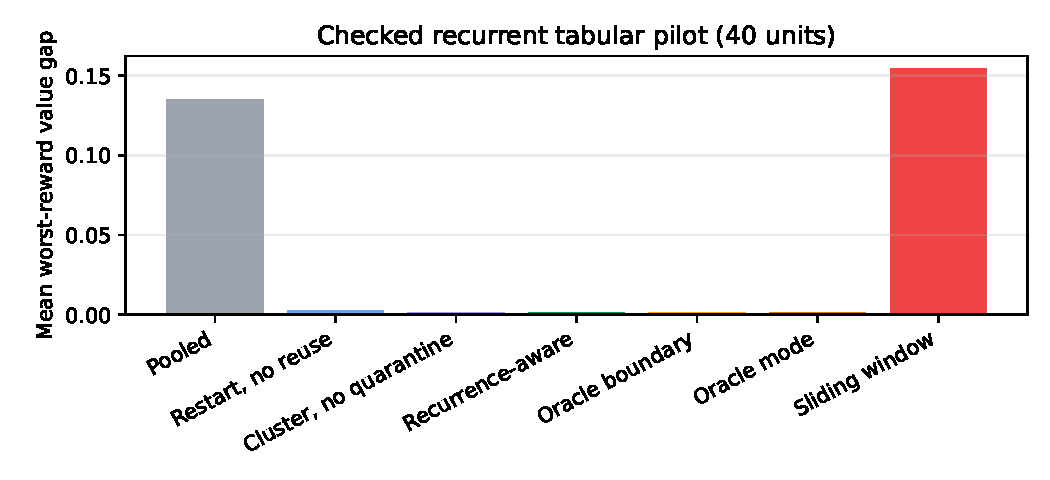
\includegraphics[width=.95\linewidth]{generated/figures/pilot_value_gaps.pdf}
\caption{Tabular mean worst-reward value gap. Lower is better.}
\label{fig:gaps}
\end{figure}

\paragraph{Tabular findings.}
Pooling and sliding windows fail when action semantics conflict across modes
(gaps $0.135$ and $0.155$). Recurrence-aware \DME{} attains gap $0.00138$,
restart attains $0.00248$, and clustering without quarantine attains
$0.00127$. Mean transition savings versus restart are $48.12$ (199 of 200
recurrence rows positive). Deployment acceptance is $1.0$ and learned mode
count is correct in all $40$ units. The paired restart-minus-\DME{}
improvement is $0.00110$, with stored seed-bootstrap $95\%$ interval
$[0.00057,0.00178]$. The interval excludes zero, but the mean is below the
predeclared $0.01$ practical margin, so the tabular gate \emph{fails}.
Clustering without quarantine is slightly better than \DME{} on this suite;
quarantine is not empirically justified here. That observation is compatible
with Theorem~\ref{thm:contam}: quarantine is a worst-case decontamination
device, and this suite may contain few mixed windows relative to dwell.
Theorem~\ref{thm:pool} explains the large pooled and sliding-window gaps:
conflicting action semantics make the mixture kernel uniformly suboptimal.

\paragraph{RFE-Recurrent-Bench.}
Because the original synthetic suite saturates restart, we added a generative
benchmark of four short-dwell tasks: a conflicting-action chain, RiverSwim with
a reversed current, a DeepSea-style dive-action swap, and Four Rooms with
moving doors. Collection remains reward-free. Hash
\texttt{90f18f4bd17c4218}, ten seeds, $40$ units
(Table~\ref{tab:bench} and Figure~\ref{fig:bench}).

The implemented detector originally almost never fired, so \DME{} collapsed to
pooling. After correcting the two-window threshold, cooldown, and adding an
active-mode residual test, recurrence-aware \DME{} attains mean gap $0.070$
versus $0.143$ for restart, $0.333$ for pooling, and $0.026$ for oracle-mode.
The paired restart-minus-\DME{} improvement is $0.073$ (bootstrap $95\%$
interval $[0.040,0.109]$), above the predeclared $0.01$ margin, so the
benchmark gate \emph{passes}. Swap-chain and DeepSea are near the oracle.
RiverSwim still pays a quarantine cost relative to clustering without
quarantine ($0.164$ versus $0.094$). The implementation now rolls back the
pre-alarm tail so mixed counts do not remain in the library; those runs are
a new protocol and do not overwrite hash \texttt{90f18f4bd17c4218}.
Tabular Four Rooms remains easy for pooling (gap $0.005$).
Collection uses a greedy covering collector in the covering-then-plan
template of \citet{jin2020rewardfree}. A likelihood-matching baseline
(\texttt{mbcd\_like}) is included in the tabular harness as a reward-free
analogue of context detection, not as the published MBCD algorithm.

\begin{table}[t]
\centering
\caption{RFE-Recurrent-Bench, ten seeds. Lower gap is better. Generated from
\texttt{results/recurrent\_bench\_pilot/results.json}.}
\label{tab:bench}
\begin{tabular}{lcccc}
\toprule
Task & Pooled & Restart & DME & Oracle mode \\
\midrule
swap\_chain & 0.175 & 0.039 & 0.002 & 0.002 \\
riverswim & 0.515 & 0.275 & 0.164 & 0.076 \\
deepsea & 0.636 & 0.042 & 0.039 & 0.000 \\
four\_rooms & 0.005 & 0.215 & 0.076 & 0.025 \\
\bottomrule
\end{tabular}

\end{table}

\begin{figure}[t]
\centering
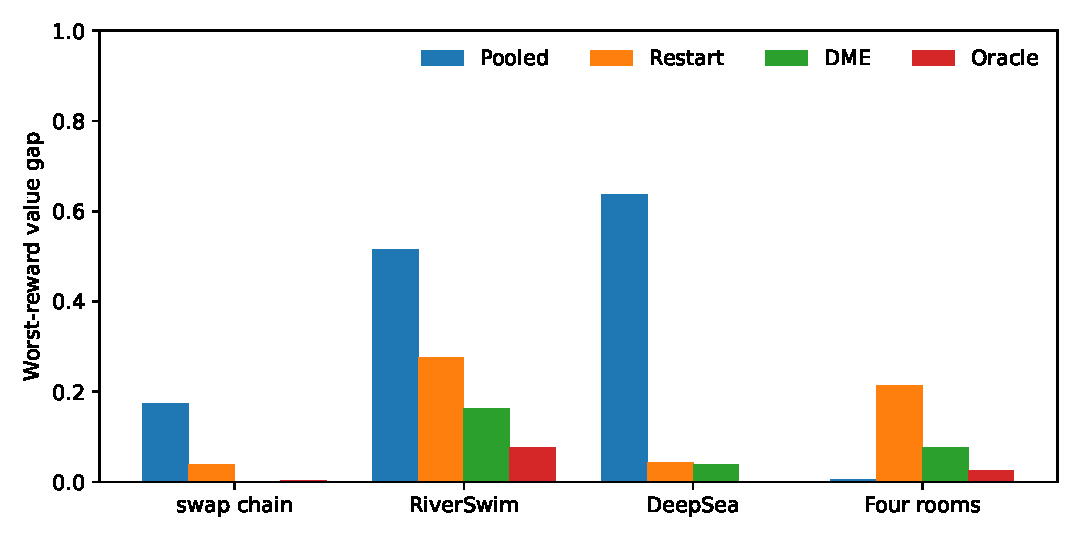
\includegraphics[width=.95\linewidth]{generated/figures/benchmark_by_task.pdf}
\caption{Per-task worst-reward gaps on RFE-Recurrent-Bench.}
\label{fig:bench}
\end{figure}

\paragraph{MiniGrid stress test.}
A ten-seed pilot uses symbolic $7\times 7$ partial observations and two
deterministic recurring transition/observation regimes
(Table~\ref{tab:minigrid}). Recurrence-aware learning has worst-task gap
$0.0492$ versus $0.2648$ for restart, saves $6.8$ samples, and has deployment
ID error $0.20$. Pooling has zero measured gap, so the scale gate fails. The
oracle is an empirical label-aware control, not an exact optimum. Observations
are symbolic, not RGB.

\begin{table}[t]
\centering
\caption{MiniGrid pilot means over ten seeds.}
\label{tab:minigrid}
\begin{tabular}{lrr}
\toprule
Method & Seeds & Mean worst-task gap \\
\midrule
pooled & 10 & 0.000000 \\
restart & 10 & 0.264844 \\
recurrence\_aware & 10 & 0.049219 \\
oracle\_upper\_bound & 10 & 0.000000 \\
\bottomrule
\end{tabular}

\end{table}

\section{Limitations}
\label{sec:limit}
The modular PAC theorem plus Theorem~\ref{thm:seg-probe} give an end-to-end
guarantee only for probe-window \DME{} with the stated window length. The
short-window residual heuristic and the greedy covering collector are not
that guarantee: covering-then-plan follows \citet{jin2020rewardfree} only
when the covering certificate meets their occupancy condition. Empirical
rewards are a finite suite. MiniGrid is too easy for pooling. Strong
separability and dwell assumptions exclude gradual drift and reward-only
changes. Wrong diagnosis can select a harmful controller; certified
abstention is required for any future deployment.

\section{Conclusion}
\label{sec:conc}
Regime-conditional RFE is a distinct objective at the intersection of
reward-free learning, recurring hidden dynamics, and active identification.
\DME{} makes the module boundaries explicit. The proved results isolate what
follows from valid segmentation and what is information-theoretically
impossible without diagnosis. Probe-window \DME{} satisfies $\SEG$ under an
explicit window length (Theorem~\ref{thm:seg-probe}); the short-window
residual heuristic used in the passing benchmark is not that theorem. The
original saturated tabular and MiniGrid gates fail. An $M$-fold direct-sum
lower bound remains open.

\appendix
\section{Notation}
\label{app:notation}
\begin{center}
\begin{tabular}{ll}
\toprule
Symbol & Meaning \\
\midrule
$S,A,H$ & state, action cardinalities and horizon \\
$P^{(m)}$ & episodic kernel of mode $m$ \\
$M_\star\le\bar M$ & unknown and known mode counts \\
$z_k,Z$ & hidden training and deployment labels \\
$q$ & diagnostic episode budget \\
$\Rone$ & rewards obeying~\eqref{eq:R} \\
$\SEG$ & segmentation contract (Definition~\ref{def:seg}) \\
$\TV,\KL,\Aff$ & total variation, KL, Hellinger affinity \\
$\mathcal{B}_q,\mathcal{K}_q^\sigma$ & controlled affinity and KL coefficients \\
$D_{\min},B$ & minimum dwell and quarantine length \\
\bottomrule
\end{tabular}
\end{center}

\section{Proofs}
\label{app:proofs}

\subsection{Proof of Lemma~\ref{lem:sim}}
Let $\tau=(s_1,a_1,\ldots,s_H,a_H)$ and write $R(\tau)=\sum_{h=1}^H r_h(s_h,a_h)$.
Condition~\eqref{eq:R} yields $R(\tau)\in[0,1]$. Let $\mu$ and $\widehat\mu$
be the laws of $\tau$ under $(P,\pi)$ and $(\widehat P,\pi)$. These laws
factor as
\[
\mu(\tau)=\rho(s_1)\prod_{h=1}^H \pi_h(a_h\mid s_h,h,\mathrm{hist})\,
P_h(s_{h+1}\mid s_h,a_h),
\]
and likewise for $\widehat\mu$, with the same $\rho$ and $\pi$. Therefore the
policies cancel in the likelihood ratio. A standard telescoping argument for trajectory laws
\citep{jaksch2010near} produces a coupling under which
\[
\TV(\mu,\widehat\mu)
\le \sum_{h=1}^H \E_{\widehat\mu}
\bigl[\TV\bigl(P_h(\cdot\mid s_h,a_h),\widehat P_h(\cdot\mid s_h,a_h)\bigr)\bigr].
\]
On the support of $\pi$ each summand is at most $\xi$, so $\TV(\mu,\widehat\mu)\le H\xi$.
For any $[0,1]$-valued random variable, $|\E_\mu R-\E_{\widehat\mu} R|\le \TV(\mu,\widehat\mu)$,
which is the value bound.

For the planning claim, let $\widehat\pi$ be optimal in $\widehat P$. Then
\begin{align*}
V_P^\star(r)-V_P^{\widehat\pi}(r)
&\le
\bigl|V_P^\star(r)-V_{\widehat P}^\star(r)\bigr|
+
\bigl(V_{\widehat P}^\star(r)-V_{\widehat P}^{\widehat\pi}(r)\bigr)
+
\bigl|V_{\widehat P}^{\widehat\pi}(r)-V_P^{\widehat\pi}(r)\bigr|.
\end{align*}
The middle term is zero. The first term is at most
$\sup_\pi |V_P^\pi(r)-V_{\widehat P}^\pi(r)|\le H\xi$ by the value bound, and
the last term is at most $H\xi$ likewise.

\subsection{Proof of Lemma~\ref{lem:chain}}
Let $X$ be the diagnostic transcript
$(s_{t,h},a_{t,h},s_{t,h+1})_{t\le q,\,h\le H}$. The strategy $\sigma$
selects $a_{t,h}$ as a (randomized) function of the strict past
$H_{t,h}$. The density of $X$ under mode $m$, with respect to a dominating
product measure, therefore factors as
\[
p_m(X)
=\prod_{t=1}^q\prod_{h=1}^H
\sigma(a_{t,h}\mid H_{t,h})\,
P_h^{(m)}(s_{t,h+1}\mid s_{t,h},a_{t,h}),
\]
and likewise for $\ell$. The factors $\sigma$ cancel in $p_m/p_\ell$. The
chain rule for KL \citep[Theorem~2.5.3]{cover2006elements} yields
\[
\KL(\mathbb{P}_m^\sigma\Vert\mathbb{P}_\ell^\sigma)
=\sum_{t,h}
\E_m\Bigl[
\KL\bigl(P_h^{(m)}(\cdot\mid s_{t,h},a_{t,h})
\Vert P_h^{(\ell)}(\cdot\mid s_{t,h},a_{t,h})\bigr)\Bigr].
\]
If a triple is never visited, the corresponding conditional KL is never
evaluated and contributes zero to the expectation. If it is visited and
$P_h^{(\ell)}(\cdot\mid s,a)$ fails to dominate $P_h^{(m)}(\cdot\mid s,a)$,
the conditional KL is $+\infty$.

\subsection{Proof of Lemma~\ref{lem:info}}
Pinsker's inequality $2\,\TV^2\le\KL$ is standard
\citep[Lemma~2.5]{tsybakov2009introduction}. Le Cam's inequality
$\TV\le\sqrt{1-\Aff^2}$ follows from writing
\[
\TV(P,Q)=\tfrac12\int |p-q|
=\tfrac12\int |\sqrt{p}-\sqrt{q}|\,|\sqrt{p}+\sqrt{q}|
\]
and Cauchy--Schwarz:
\[
\bigl(\tfrac12\int |\sqrt{p}-\sqrt{q}|\,|\sqrt{p}+\sqrt{q}|\bigr)^2
\le
\bigl(\tfrac12\int (\sqrt{p}-\sqrt{q})^2\bigr)
\bigl(\tfrac12\int (\sqrt{p}+\sqrt{q})^2\bigr)
=(1-\Aff)(1+\Aff)=1-\Aff^2.
\]
Rearrangement gives $\Aff\le\sqrt{1-\TV^2}$. The elementary bound
$1-u\le e^{-u}$ with $u=\TV^2$ yields $\sqrt{1-\TV^2}\le e^{-\TV^2/2}$.

\subsection{Proof of Theorem~\ref{thm:pool}}
Coordinatewise, $M_h(\cdot\mid s,a)-\,P_h(\cdot\mid s,a)
=(1-\alpha)\bigl(Q_h(\cdot\mid s,a)-P_h(\cdot\mid s,a)\bigr)$, so taking
$\tfrac12\|\cdot\|_1$ proves the TV identity.

For inconsistency, reuse the instance of Theorem~\ref{thm:zero}: one-step
MDP, actions $\{a_0,a_1\}$, terminals $\{g,b\}$, mode $0$ sending $a_0$ to
$g$ and $a_1$ to $b$, mode $1$ reversed, and $r(g)=1$. The mixture
$M=\tfrac12 P^{(0)}+\tfrac12 P^{(1)}$ sends both actions to $g$ with
probability $1/2$. Every policy is optimal for $M$ and has value $1/2$ in
both true modes, while $V^\star=1$. Infinite mixed data recover $M$ exactly
and still yield gap $1/2$.

\subsection{Proof of Theorem~\ref{thm:contam}}
Condition on the $n$ mode labels in the window and on the (predictable)
policies. Each accepted transition at a fixed $(h,s,a)$ is drawn from
$P_h$ or $Q_h$ according to the episode's mode. The empirical next-state
frequency is the corresponding mixture of empirical measures, whose
conditional expectation is the displayed convex combination. Taking
$\TV(\cdot,P_h)$ and using Theorem~\ref{thm:pool} with
$\alpha=n_0/n$ gives the bias identity. If every episode whose window
straddles a true boundary lies in the $B$ episodes at each block end, those
episodes are excluded from accepted counts and the identity is never
applied to a mixed window.

\subsection{Proof of Lemma~\ref{lem:match}}
Write $d_\infty(P,Q)=\max_{h,s,a}\TV(P_h,Q_h)$. By assumption
$d_\infty(P^{(m)},P^{(\ell)})\ge\Delta$ for $m\neq\ell$. A TV-ball of
radius $\rho<\Delta/4$ around $P^{(m)}$ is disjoint from the ball of radius
$\rho$ around $P^{(\ell)}$, and the gap between balls is greater than
$\Delta/2$. Hence if $\cC_{\mathrm{new}}$ and $\cC_i$ are balls of radius
$\rho$ around the same kernel, $d_i=0$; if they wrap distinct kernels,
$d_i>\Delta/2=\gamma$. Algorithm~2 therefore returns the unique true index
on a recurrence and \textsc{New} on an unseen separated mode. If radii
fail to be valid, the lemma does not apply.

\subsection{Proof of Lemma~\ref{lem:account}}
Under $\SEG$, each of the $J$ blocks contributes at most $2B$ quarantined
episodes and therefore at least $D_{\min}-2B$ accepted episodes, all
assigned to the same library index. Restart that keeps only the last block
has at most $D_{\min}$ episodes (even without quarantine). The comparison
$D_{\min}<N\le J(D_{\min}-2B)$ is arithmetic.

\subsection{Proof of Theorem~\ref{thm:modular}}
Let $E_{\mathrm{seg}}$ be the $\SEG$ event, $E_m$ the success of the
stationary RFE call for mode $m$, and $E_{\mathrm{id}}$ correct deployment
identification. The hypotheses are
$\Prb(E_{\mathrm{seg}}^c)\le\deltaseg$,
$\Prb(E_m^c\mid E_{\mathrm{seg}})\le\deltarfe$, and
$\Prb(E_{\mathrm{id}}^c\mid E_{\mathrm{seg}}\cap\bigcap_m E_m)\le\deltaid$.
A union bound gives
\[
\Prb\Bigl(E_{\mathrm{seg}}\cap\bigcap_{m=1}^{M_\star}E_m\cap E_{\mathrm{id}}\Bigr)
\ge 1-\deltaseg-M_\star\deltarfe-\deltaid.
\]
On this intersection, Definition~\ref{def:seg} supplies a bijection from
library indices to true modes, every accepted sample is pure, each planner
$\Pi_i$ is uniformly $\eta$-accurate for its kernel, and $\widehat m$ equals
the library index of $Z$. Therefore
$\sup_{r\in\Rone}\mathrm{gap}(r)\le\eta$.

\subsection{Proof of Theorem~\ref{thm:decomp}}
On $G\cap\{\widehat m=Z\}$ the gap is at most $\eta$ uniformly in $r$. On the
complement the gap is at most $1$ by~\eqref{eq:R}. Hence
\[
\E[\mathrm{gap}(r)]
\le \eta\,\Prb(G\cap\{\widehat m=Z\})
+ 1\cdot\Prb(G^c\cup\{\widehat m\neq Z\}).
\]
The event $G^c\cup\{\widehat m\neq Z\}$ is contained in
$G^c\cup\bigl(G\cap\{\widehat m\neq Z\}\bigr)$, which has probability at most
$\alpha+\beta$. The same inclusion yields the high-probability bound because
on $G\cap\{\widehat m=Z\}$ one has $\sup_r\mathrm{gap}(r)\le\eta$.

\subsection{Proof of Corollary~\ref{cor:rate}}
Apply Theorem~\ref{thm:modular} with the given quotas. The inclusion
$\Rone\subset\{r:r_h\in[0,1]\}$ is immediate from~\eqref{eq:R}, so any
guarantee stated for the larger class remains valid on $\Rone$ at the same
$\eta$. The warning about sampling interfaces is the content of
Definition~\ref{def:seg}(iv): purity does not imply that a published RFE
theorem applies.

\subsection{Proof of Proposition~\ref{prop:aff}}
Let $p_j$ be densities of $\mathbb{P}_j^\sigma$ under a common dominating
measure. Maximum likelihood errs in favour of $\ell$ only on
$\{p_\ell\ge p_m\}$, and
\[
\Prb_m(p_\ell\ge p_m)
=\int_{\{p_\ell\ge p_m\}} p_m
\le \int \sqrt{p_m p_\ell}
=\Aff(\mathbb{P}_m^\sigma,\mathbb{P}_\ell^\sigma),
\]
because $p_m\le\sqrt{p_m p_\ell}$ on that set. A union bound over
$\ell\neq m$ proves the claim. Writing $\Aff=\exp(\log\Aff)$ gives the
exponential form.

\subsection{Proof of Theorem~\ref{thm:known-rate}}
Fix a distinguishing triple $(h^\star,s^\star,a^\star)$ at which two
candidates differ by TV at least $\Delta$. Let $N$ be the number of
diagnostic visits to that triple over $q$ episodes. Each episode contributes
a visit with probability at least $\mu$, so $N$ stochastically dominates
$\mathrm{Bin}(q,\mu)$. A Chernoff bound yields
$\Prb(N<\mu q/2)\le\exp(-\mu q/8)$.

On the event $\{N\ge \mu q/2\}$, let $\widehat p$ be the empirical next-state
distribution at the triple. The test returns the unique library kernel whose
TV distance to $\widehat p$ is at most $\Delta/4$, and rejects if none or
several exist. If the truth $P^{(m)}$ satisfies $\TV(\widehat p,P^{(m)})\le\Delta/4$,
then every competitor $P^{(\ell)}$ has
$\TV(\widehat p,P^{(\ell)})\ge\Delta-\Delta/4=3\Delta/4$, so the test is
correct.

Weissman's inequality \citep{weissman2003inequalities} gives, for an alphabet
of size $S$,
\[
\Prb\bigl(\TV(\widehat p,P^{(m)})>\Delta/4\mid N=n\bigr)
\le (2^S-2)\exp\bigl(-2n(\Delta/4)^2\bigr)
=(2^S-2)\exp(-n\Delta^2/8).
\]
Choosing
$q\ge (32/(\mu\Delta^2))\bigl(S\log 2+\log(4\bar M/\deltaid)\bigr)$
makes $\mu q/2\ge (16/\Delta^2)(S\log 2+\log(4\bar M/\deltaid))$, hence
\[
\exp(-\mu q/8)\le \frac{\deltaid}{4\bar M},
\qquad
(2^S)\exp(-(\mu q/2)\Delta^2/8)\le\frac{\deltaid}{4\bar M}.
\]
A union bound over at most $\bar M$ candidates completes the proof.

\subsection{Proof of Lemma~\ref{lem:twowindow}}
Let $\nu$ be the common law of a pure same-mode window of length $n$. Then
\[
\TV(\widehat\nu_{\mathrm{L}},\widehat\nu_{\mathrm{R}})
\le \TV(\widehat\nu_{\mathrm{L}},\nu)+\TV(\widehat\nu_{\mathrm{R}},\nu).
\]
A false alarm requires the left-hand side to exceed $\Delta/2$, hence some
window to have TV error greater than $\Delta/4$. Weissman's inequality yields
\[
\Prb\bigl(\TV(\widehat\nu,\nu)>\Delta/4\bigr)
\le (2^d-2)\exp(-n\Delta^2/8).
\]
For two windows and $T$ split times, the union bound is at most
$2T(2^d)\exp(-n\Delta^2/8)$. The stated $n$ makes this at most $\delta$.

If the two windows are pure and drawn from laws at TV distance at least
$\Delta$, the same decomposition gives
$\TV(\widehat\nu_{\mathrm{L}},\widehat\nu_{\mathrm{R}})
\ge\Delta-\TV(\widehat\nu_{\mathrm{L}},\nu^{(m)})-\TV(\widehat\nu_{\mathrm{R}},\nu^{(\ell)})$.
Both empirical errors being at most $\Delta/4$ produces an alarm. The failure
probability is therefore controlled by the same estimate.

\subsection{Proof of Theorem~\ref{thm:seg-probe}}
Write $\delta=\deltaseg$. Apply Lemma~\ref{lem:twowindow} to the probe-episode
stream with failure probability $\delta/4$ and $T$ candidate splits. On that
event: (i)~no pair of pure same-mode windows of length $n$ alarms;
(ii)~every pair of pure different-mode windows of length $n$ alarms, so after
a switch the delay is at most $n$ once both windows are pure.

Rollback removes the last $n$ accepted probe episodes from the active library
at the alarm. Quarantine then discards $n$ post-alarm episodes. Hence mixed
windows are contained in the last $n$ episodes of the old block and the first
$n$ of the new block, which is localization with $B=n$. Accepted interiors
are therefore pure, which is (i) in Definition~\ref{def:seg}.

Confirmation windows of length at least $n$ yield empirical laws within TV
distance $\rho=\Delta/4$ of the true probe law, again by Weissman and a union
bound of $\delta/4$ over at most $J$ segments. Lemma~\ref{lem:match} with
$\gamma=\Delta/2$ therefore returns a unique recurrence or \textsc{New}, which
is (iii). Weissman balls of radius $\rho$ about the pooled accepted probe
counts cover the true kernels jointly with probability $1-\delta/4$ over at
most $\bar M\,d$ coordinates, which is (v).

Assumption~\ref{ass:dwell} with $B=n$ yields at least
$D_{\min}-2n$ accepted episodes per block. Recurrence pooling and
Assumption~\ref{ass:occ} give the RFE quota (iv). A union bound of four
$\delta/4$ events completes $\SEG(n,\mathbf{n},\delta)$.

The argument uses i.i.d.\ probe episodes. It does not apply to a residual
detector run on an adaptive RFE policy in a continuing MDP, nor to a TV
threshold smaller than $\Delta/2$ with $n$ below the displayed length.

\subsection{Proof of Proposition~\ref{prop:robust}}
On the event that each $\cC_i$ is a TV ball of radius $\rho$ about the truth,
any empirical diagnostic law $\widehat\nu$ with
$\TV(\widehat\nu,P^{(m)})\le(\Delta-2\rho)/4$ lies at distance at most
$\Delta/2-\rho$ from the true ball and at least $3\Delta/4-\rho$ from every
competitor ball. The threshold $\Delta/2-\rho$ therefore separates them.
Theorem~\ref{thm:known-rate} applies with $\Delta\leftarrow\Delta-2\rho$.

\subsection{Proof of Theorem~\ref{thm:zero}}
Consider a one-step problem with initial state $x$, actions $\{a_0,a_1\}$, and
terminals $\{g,b\}$. In mode $0$, $a_0$ leads to $g$ and $a_1$ to $b$; in
mode $1$ the transitions are reversed. Let $r$ assign $1$ at $g$ and $0$
elsewhere, which satisfies~\eqref{eq:R}. With $q=0$ the algorithm must choose
a (possibly randomized) action at $x$ independently of the deployment label.
If it selects $a_0$ with probability $p$, the losses are $1-p$ and $p$. Their
maximum is at least $1/2$. Both modes may have appeared arbitrarily often
during training; the missing information is which one is deployed.

\subsection{Proof of Theorem~\ref{thm:diag-lb}}
For binary hypotheses,
$\inf_\psi(\Prb_m(\psi=\ell)+\Prb_\ell(\psi=m))
=1-\TV(\mathbb{P}_m^\sigma,\mathbb{P}_\ell^\sigma)$
\citep{lecam1973convergence}. Bretagnolle--Huber
\citep{bretagnolle1978estimation,canonne2023short} gives
$\TV\le\sqrt{1-e^{-\KL}}$. Set $x=e^{-\KL}\in[0,1]$. The inequality
$1-\sqrt{1-x}\ge x/2$ holds because
$f(x)=1-\sqrt{1-x}-x/2$ satisfies $f(0)=0$ and
$f'(x)=\tfrac12(1-x)^{-1/2}-1/2\ge 0$ on $[0,1)$. Therefore
$1-\TV\ge \tfrac12 e^{-\KL}$. Under equal priors the error probability is
at most half of the two-hypothesis sum and at least half of its infimum;
multiplying the infimum by $\gamma/2$ (the equal-prior mixture of the two
directional losses) yields the regret bound
$\tfrac{\gamma}{4}\exp(-\KL)$.

\subsection{Proof of Theorem~\ref{thm:occupancy}}
We give a self-contained two-action construction. Let $H=1$, with initial
state $x$, actions $\{a_+,a_-\}$, and terminals $\{g,b\}$. Mode $0$ is
deterministic: both actions lead to $g$. Mode $\theta\in\{+\gamma,-\gamma\}$
has
\[
P(g\mid x,a_+)=\tfrac12+\theta,\qquad
P(g\mid x,a_-)=\tfrac12-\theta,
\]
with $0<\gamma\le 1/4$. Let $r$ assign $1$ at $g$ and $0$ at $b$, which lies
in $\Rone$. Then $V^\star=1/2+\gamma$ and the suboptimal action has gap
$2\gamma$.

Take $\gamma=\eps$ with $\eps<1/8$, so a wrong action has gap $2\eps>\eps$.
The common mode is uninformative about $\theta$. All information about the
rare mode is contained in its $N_0$ episodes. Each episode, under any
action, yields a Bernoulli observation whose KL between $+\gamma$ and
$-\gamma$ is at most $\chi^2=4\gamma^2/(\tfrac14-\gamma^2)\le 32\gamma^2$
for $\gamma\le 1/4$. Thus
$\mathcal{K}_{N_0}\le 32 N_0\eps^2$. Theorem~\ref{thm:diag-lb} yields
two-hypothesis error at least $\tfrac12\exp(-32 N_0\eps^2)$. If
$N_0\le (1/32)\eps^{-2}\log 2$, this is at least $1/4$. Any algorithm that
then selects an action for the rare mode therefore has
$\Prb(\mathrm{gap}>\eps)\ge 1/4$, so it cannot be $(\eps,\delta)$-PAC for
$\delta<1/8$.

\subsection{Proof of Theorem~\ref{thm:behavior}}
If two kernels induce the same law under every policy, the observed training
and diagnostic transcripts are identically distributed, so any test has error
at least $1/2$ in the two-hypothesis problem. Values coincide because they are
expectations of~\eqref{eq:R} under those laws. Conversely, if
$P_h^{(m)}(\cdot\mid s,a)\neq P_h^{(\ell)}(\cdot\mid s,a)$ and some policy
reaches $(s,a)$ at step $h$ with positive probability from $\rho$, then the
one-step KL at that triple is strictly positive (or infinite). Lemma~\ref{lem:chain}
therefore yields $\mathcal{K}_q^\sigma(m,\ell)>0$ for a strategy that targets
the triple, hence $\mathcal{B}_q>0$.

\section{Reproducibility}
\label{app:repro}
From the repository root:
\begin{verbatim}
python3 -m pytest -q
python3 run.py --protocol recurrent-tabular --profile pilot \
  --output results/recurrent_tabular_pilot
python3 run.py --protocol minigrid-recurrent --profile pilot \
  --output results/minigrid_recurrent_pilot
python3 run.py --protocol recurrent-bench --profile pilot \
  --output results/recurrent_bench_pilot
python3 scripts/generate_regime_rfe_assets.py
python3 scripts/generate_benchmark_assets.py
tectonic paper/regime_rfe.tex --keep-logs
\end{verbatim}
Tables and figures are generated from retained JSON/CSV. The official NeurIPS
style file was unavailable locally; the compiled PDF uses the declared article
fallback.

\bibliographystyle{plainnat}
\bibliography{regime_rfe_references}
\end{document}
